\section{Implementations-Sicht}
\label{sec:sad-implementation}

\subsection{Rendering des User Interfaces und Event-Behandlung}
Durch die Verwendung von \emph{barefoot} \cite{Barefoot} kann die komplette Beispielapplikation sowohl eigenständig auf dem Server gerendert werden, als auch als moderne JavaScript Applikation im Browser des Endbenutzers ausgeführt werden. Aus diesem Grund zeigen die folgenden zwei Abschnitte jeweils ein separates Sequenzdiagramm: Eines für das Event-Handling auf dem Client und eines für den Rendering-Vorgang auf dem Server.

Grundlegende Unterschiede gibt es hierbei lediglich beim Zugriff auf den \emph{APIAdapter}. Auf dem Server werden diese direkt lokal behandelt, im Client-Browser wird die entsprechende API-Abfrage über einen HTTP REST Request übertragen.

\subsubsection*{Server}
Beim initialen Aufruf der Beispielapplikation werden die kompletten Inhalte des User Interfaces auf dem Server gem. Diagramm \ref{dig:serverrendering} gerendert. Sollte der Client-Browser zudem JavaScript deaktiviert haben oder nicht unterstützen, so werden auch nachfolgende Requests nach dem gleichen Schema verarbeitet und gerendert.

\begin{figure}[H]
	\centering{
		\resizebox{0.9\textwidth}{!} {
			\begin{tikzpicture}
				\begin{umlseqdiag}
					\umlactor[class=Browser, fill=white]{client}
					\umlboundary[class=ExpressJS, fill=white]{app}
					\umlobject[class=Router, fill=sharedColor!20]{router}
					\umlobject[class=View, fill=sharedColor!20]{view}
					\umlobject[class=Model, fill=sharedColor!20]{model}
					\umlobject[class=ApiAdapter, fill=apiColor!20]{apiAdapter}
					\umlobject[class=DataStore, fill=barefootColor!20]{dataStore}

					\begin{umlcall}[op={Click -> Request}, return=HTML]{client}{app}
						\begin{umlcall}[op=route(), with return]{app}{router}
							\begin{umlcallself}[op=render()]{router}
								\begin{umlcallself}[op=initDOM()]{router}
								\end{umlcallself}
								\begin{umlcallself}[op=renderMainView()]{router}
								\end{umlcallself}

								\begin{umlcallself}[op=renderView()]{router}
									\begin{umlcall}[op=beforeRender(), with return]{router}{view}
										\begin{umlcall}[op={fetch()}, return=success()]{view}{model}
											\begin{umlcall}[op={sync()}, return=success()]{model}{apiAdapter}
											\end{umlcall}
										\end{umlcall}
									\end{umlcall}

									\begin{umlcall}[op=renderView(), return=HTML]{router}{view}
									\end{umlcall}

									\begin{umlcall}[op=afterRender(), with return]{router}{view}
									\end{umlcall}
								\end{umlcallself}

								\begin{umlcall}[op=toJSON(), with return]{router}{dataStore}
								\end{umlcall}

								\begin{umlcallself}[op=writeHTTPResponse()]{router}
								\end{umlcallself}
							\end{umlcallself}
						\end{umlcall}
					\end{umlcall}
				\end{umlseqdiag}
			\end{tikzpicture}
		}
	}
	\caption{Sequenzdiagramm: Rendering und Event-Verarbeitung auf dem Server}
	\label{dig:serverrendering}
\end{figure}

\subsubsection*{Client}
Das Sequenzdiagramm \ref{dig:clientrendering} zeigt den Kontrollfluss nachdem der Benutzer im Browser auf einen Eintrag im Navigationsmenü geklickt hat.

Es gilt zu beachten dass die Aufrufe auf den \emph{APIAdapter} nicht lokal verarbeitet werden sondern direkt auf dem Server.

\begin{figure}[H]
	\centering{
		\resizebox{0.9\textwidth}{!} {
			\begin{tikzpicture}
				\begin{umlseqdiag}
					\umlactor[class=Browser]{client}
					\umlobject[class=View]{current}
					\umlobject[class=Router]{router}
					\umlobject[class=View]{next}
					\umlobject[class=Model]{model}
					\umlobject[class=Backbone]{backbone}
					\umlobject[class=ApiAdapter]{apiAdapter}

					\begin{umlcall}[op=Click Menu Item, with return]{client}{current}
						\begin{umlcall}[op=navigate(), with return]{current}{router}
							\begin{umlcallself}[op=render()]{router}
								\begin{umlcallself}[op=renderView()]{router}
									\begin{umlcall}[op=beforeRender(), with return]{router}{next}
										\begin{umlcall}[op={fetch()}, return=success()]{next}{model}
											\begin{umlcall}[op={sync()}, return=success()]{model}{backbone}
												\begin{umlcall}[op={HTTP REST Request}, return=HTTP Response]{backbone}{apiAdapter}
												\end{umlcall}
											\end{umlcall}
										\end{umlcall}
									\end{umlcall}

									\begin{umlcall}[op=renderView(), return=HTML]{router}{next}
									\end{umlcall}

									\begin{umlcall}[op=afterRender(), with return]{router}{next}
									\end{umlcall}
								\end{umlcallself}

								\begin{umlcallself}[op=Replace DOM Element]{router}
								\end{umlcallself}
							\end{umlcallself}
						\end{umlcall}
					\end{umlcall}
				\end{umlseqdiag}
			\end{tikzpicture}
		}
	}
	\caption{Sequenzdiagramm: Rendering und Event-Verarbeitung auf dem Client}
	\label{dig:clientrendering}
\end{figure}



\subsection{APIAdapter}
Wie bereits erwähnt kann der \emph{APIAdapter} auf dem Server sowohl mit server-lokalen Requests als auch mit HTTP REST Anfragen umgehen.

Das Diagramm \ref{dig:apiAdapter} verdeutlicht die Abläufe im innern des Adapters für den jeweiligen Anfragemodus.

Hinter dem Element \emph{Controllers} stehen neben dem eigentlichen API-Controller zusätzlich diverse Sicherheitspolicies und Validatoren, welche eingehende Requests prüfen und ggf. abweisen können, bevor sie zur eigentlichen Geschäftslogik gelangen.

\begin{figure}[H]
	\centering{
		\resizebox{0.9\textwidth}{!} {
			\begin{tikzpicture}
				\begin{umlseqdiag}
					\umlactor[class=Caller]{caller}
					\umlboundary[class=ExpressJS]{app}
					\umlobject[class=APIAdapter]{apiAdapter}
					\umlmulti[class=Controllers]{controller}
					\umldatabase[class=Persistency]{db}

					\begin{umlfragment}[type=alt, label={Server-local}, inner xsep=12]
						\begin{umlcall}[op={sync()}, return={success()}, dt=8]{caller}{apiAdapter}
							\begin{umlcallself}[op={dispatchLocalApiCall()}]{apiAdapter}
							\end{umlcallself}
							\begin{umlcallself}[op={processCallbacks()}]{apiAdapter}
							\end{umlcallself}
							\begin{umlcall}[op={handler()}, return={success()}]{apiAdapter}{controller}
								\begin{umlcall}[op={consume}, with return]{controller}{db}
								\end{umlcall}
							\end{umlcall}
						\end{umlcall}

						\umlfpart[HTTP REST]

						\begin{umlcall}[op={HTTP Request}, return={JSON Response}]{caller}{app}
							\begin{umlcallself}[op={Dispatch}]{app}
							\end{umlcallself}
							\begin{umlcall}[op={handler()}, return={JSON Object}]{app}{apiAdapter}
								\begin{umlcallself}[op={processCallbacks}]{apiAdapter}
								\end{umlcallself}
								\begin{umlcall}[op={handler()}, return={success()}]{apiAdapter}{controller}
									\begin{umlcall}[op={consume}, with return]{controller}{db}
									\end{umlcall}
								\end{umlcall}
							\end{umlcall}
						\end{umlcall}
					\end{umlfragment}

				\end{umlseqdiag}
			\end{tikzpicture}
		}
	}
	\caption{Sequenzdiagramm: APIAdapter im server-lokalen sowie HTTP REST Modus}
	\label{dig:apiAdapter}
\end{figure}


\subsection{Quellcode Organisation}
\gls{nodejs} Applikationen werden üblicherweise soweit wie möglich in eigenständige und wiederverwendbare Komponenten (siehe \cite{TJH_ComponentStructure} und \cite{IZS_ComponentStructure}) aufgeteilt.

Ein gutes Beispiel hierfür ist die Vielzahl an verfügbaren Modulen welche über den Komponentenmanager NPM \cite{NPM} installierbar sind. Selbst Bibliotheken mit minimalem Umfang werden und sollten als eigene Module gekappselt werden.

Die Beispielapplikation ``Roomies'' verwendet selber mehrere Komponenten aus NPM \cite{NPM} und ist selber in Komponenten unterteilt. Dies veranschaulicht die Ordnerstruktur in Abbildung \ref{fig:roomiesFolderStructure}.

\newpage
\subsubsection*{Ordnerstruktur}

\begin{figure}[H]
	\centering
	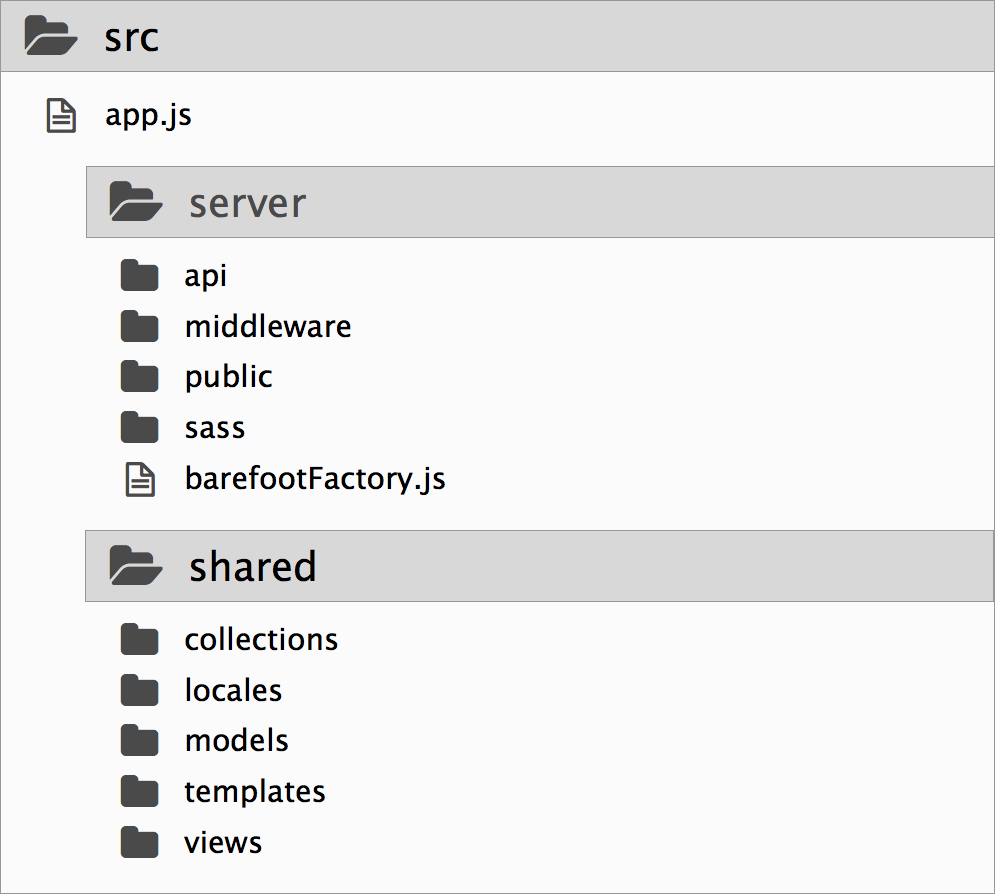
\includegraphics[width=8cm]{content/sad/images/folder-structure.png}
	\caption{Ordnerstruktur des \emph{src}-Unterordners der Beispielapplikation \emph{Roomies}}
	\label{fig:roomiesFolderStructure}
\end{figure}

Jede Komponente mit JavaScript-Code kann mittels einem ``require()''-Befehl eingebunden werden. Zu diesem Zweck wird jeweils nur der Ordnername angegeben. Damit wird automatisch die enthaltene index.js-Datei geladen.


\begin{lstlisting}[language=JavaScript, caption=Einbindung der Community-Komponente, float=ht!]
// Requires actually src/server/api/community/index.js:
// Found in src/server/api/index.js
var setupCommunityApi = require('./community');
\end{lstlisting}

Im folgenden werden die beiden wichtigsten Dateien für das Starten der Applikation erklärt.

\subsubsection*{barefootFactory.js}
Die ``barefoot''-Factory \cite{barefootFactoryjs} ist verantwortlich für das Setup der Server-Seite der Applikation.
Unter anderem werden folgende wichtige Aufgaben ausgeführt:
\begin{itemize}
	\item{Definition der JavaScript Dateien, die am Client geschickt werden sollen}
	\item{Einrichtung der API-Adapter}
	\item{Laden der Express.js \cite{Expressjs} Middleware}
	\item{Starten des Express.js \cite{Expressjs} HTTP Servers}
	\item{Einrichten des Server Request Contexts (u.a. das Model für den eingeloggten Benutzer).}
\end{itemize}

Diese Informationen werden ``barefoot'' \cite{Barefoot} mitgegeben, damit das Framework weiss, was zu starten ist.

\subsubsection*{app.js}
Die Datei ``app.js'' \cite{appjs} ist der Startpunkt der Applikation.
Darin wird u.a. die ``barefootFactory'' instanziert und der ``DataStore'' initialisiert.

Der ``DataStore'' ist ein ``barefoot'' Konzept (siehe \cite{barefootDatastore}). Es wird verwendet um Models und Collections vom Server zum Client zu senden.